\documentclass[a4paper,12pt]{article}

% PACOTES
\usepackage[portuguese]{babel}
\usepackage[utf8]{inputenc}
\usepackage[T1]{fontenc}
\usepackage[a4paper,top=2cm,bottom=2cm,left=3cm,right=3cm]{geometry}
\usepackage{graphicx}          % para inserir imagens
\usepackage{amsmath}           % símbolos matemáticos
\usepackage[colorlinks=true,
            linkcolor=red,        % cor dos links internos
            urlcolor=blue,         % cor dos links externos
            ]{hyperref}  
\usepackage{listings}          % para inserir código
\usepackage{xcolor}            % cores no código
\usepackage{indentfirst}

\usepackage[backend=biber, style=ieee]{biblatex}
\usepackage{tikz}
\usetikzlibrary{positioning, arrows.meta}
\addbibresource{referencias.bib} % Substituir por nome exato do ficheiro .bib

% CONFIGURAÇÃO DE CÓDIGO (Python, Bash, C++)
\definecolor{codegreen}{rgb}{0,0.6,0}
\definecolor{codegray}{rgb}{0.5,0.5,0.5}
\definecolor{codepurple}{rgb}{0.58,0,0.82}
\definecolor{backcolour}{rgb}{0.95,0.95,0.92}

\lstset{
    backgroundcolor=\color{backcolour},   
    commentstyle=\color{codegreen},
    keywordstyle=\color{magenta},
    numberstyle=\tiny\color{codegray},
    stringstyle=\color{codepurple},
    basicstyle=\ttfamily\footnotesize,
    breakatwhitespace=false,         
    breaklines=true,                 
    captionpos=b,                    
    keepspaces=true,                 
    numbers=left,                    
    numbersep=5pt,                  
    showspaces=false,                
    showstringspaces=false,
    showtabs=false,                  
    tabsize=2,
    literate=
     {á}{{\'a}}1 {à}{{\`a}}1 {ã}{{\~a}}1 {â}{{\^a}}1 {Á}{{\'A}}1 {À}{{\`A}}1 {Ã}{{\~A}}1 {Â}{{\^A}}1
     {é}{{\'e}}1 {è}{{\`e}}1 {ê}{{\^e}}1 {É}{{\'E}}1 {È}{{\`E}}1 {Ê}{{\^E}}1
     {í}{{\'i}}1 {ì}{{\`i}}1 {î}{{\^i}}1 {Í}{{\'I}}1 {Ì}{{\`I}}1 {Î}{{\^I}}1
     {ó}{{\'o}}1 {ò}{{\`o}}1 {õ}{{\~o}}1 {ô}{{\^o}}1 {Ó}{{\'O}}1 {Ò}{{\`O}}1 {Õ}{{\~O}}1 {Ô}{{\^O}}1
     {ú}{{\'u}}1 {ù}{{\`u}}1 {û}{{\^u}}1 {Ú}{{\'U}}1 {Ù}{{\`U}}1 {Û}{{\^U}}1
     {ç}{{\c{c}}}1 {Ç}{{\c{C}}}1,
    extendedchars=true
}

% INFORMAÇÕES DO TRABALHO
\title{\textbf{Automação II}}
\author{Tomás Espincho -- 110486}
\date{\today}

\setlength{\parindent}{1.25cm}

\begin{document}

% CAPA
\begin{titlepage}
    \centering

\noindent
    \hfill
    
\includegraphics[width=0.30\textwidth]{./img/LogoUA.png}

    {\Huge \textbf{Projeto Automação II}}\\[1cm]
    {\large Licenciatura em Automação Industrial}\\[2cm]

    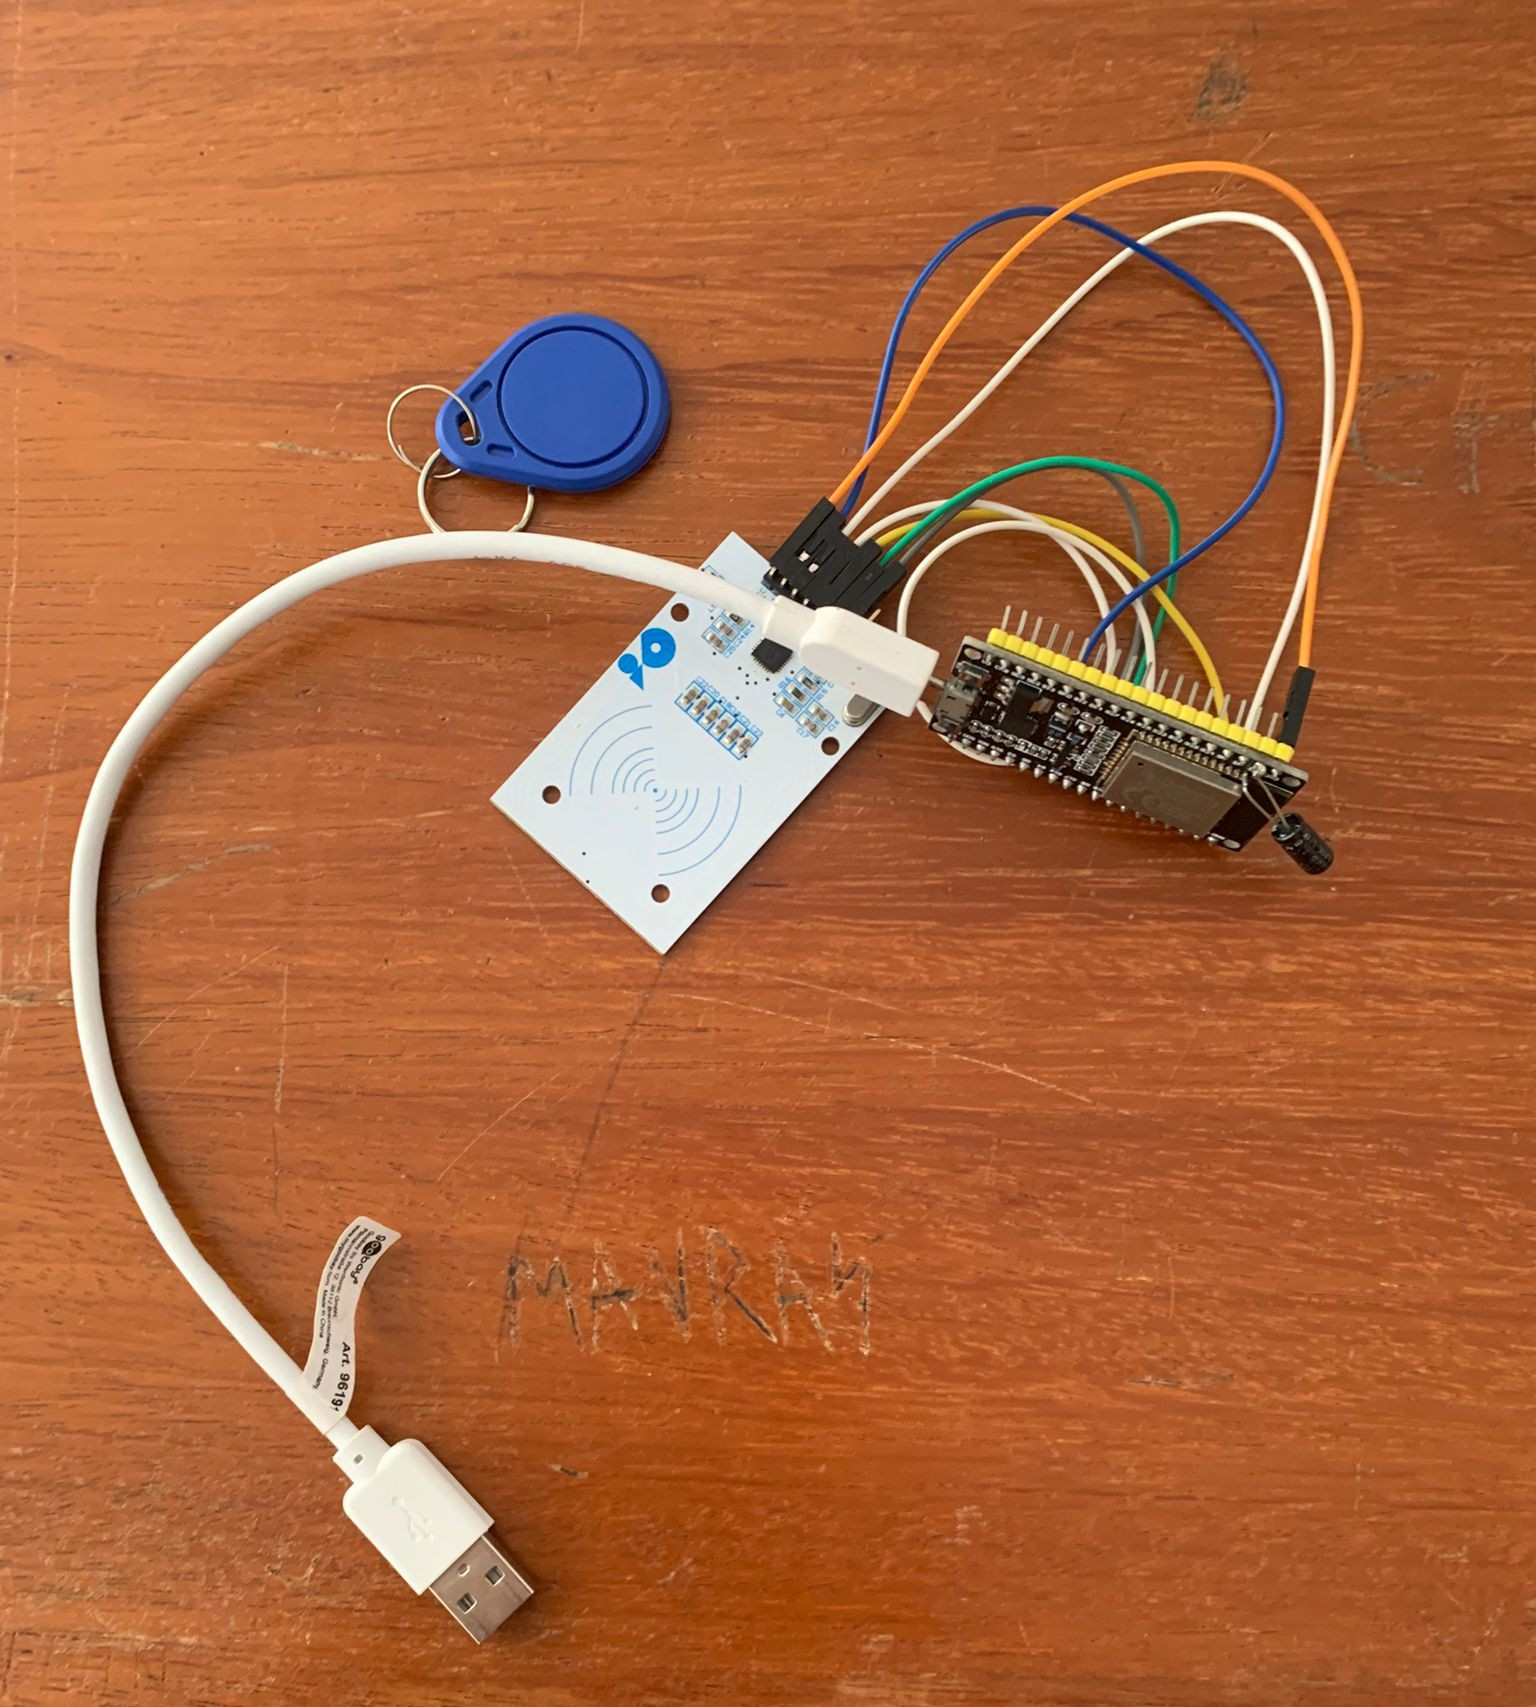
\includegraphics[width=0.9\textwidth]{./img/capa.jpeg}
    \vfill

    {\Large Tomás Espincho (110486)}\\[0.5cm]

    {\large \today}\\[2cm]

\end{titlepage}

% INÍCIO DO TRABALHO
\newpage
\tableofcontents
\newpage

\section{Introdução}

Neste projeto, o objetivo consiste em desenvolver um programa que lê uma tag RFID e a publica num broker MQTT. A arquitetura principal baseia-se num leitor RFID (MFRC522) ligado a um ESP32, que comunica com o servidor MQTT por Wi-Fi e, no Docker para alojar os serviços do broker e da dashboard.  

O processo começa por ler uma tag RFID. O ESP32 usa a biblioteca MFRC522.h para extrair o UID e a biblioteca NTPClient para registar a hora exata da leitura. Depois, esta informação é estruturada num JSON e enviada para o broker MQTT. Por fim, o broker envia a informação para todos os subscritores do tópico, seja o script Python ou a dashboard.

\section{Explicação do Código}
O código desenvolvido neste trabalho é apresentado e explicado nas subsecções seguintes, divididas por linguagem de programação.

\subsection{Código do ESP32}

O código do ESP32 é responsável pela interação com o leitor RFID, processamento dos dados e comunicação MQTT. O código completo encontra-se disponível no repositório GitHub e(ou) no zip do projeto. Nesta secção, estão apenas explicitas as partes mais estroturais do codigo.

\subsubsection{Conversão do UID para Hexadecimal}

Após a leitura de uma tag, o UID é obtido como um \textit{array} de \textit{bytes}. Para garantir a correta formatação dos dados no sistema, este valor é convertido numa \textit{string} em formato hexadecimal.

A lógica do módulo baseia-se na documentação e exemplos práticos do sensor RC522 \cite{instructables_rc522_arduino, youtube_rfid_rc522}

\begin{lstlisting}[language=C++, caption={Conversão do UID para formato hexadecimal}]
String tagUID = "";
for (byte i = 0; i < mfrc522.uid.size; i++) {
  tagUID.concat(String(mfrc522.uid.uidByte[i] < 0x10 ? " 0" : " "));
  tagUID.concat(String(mfrc522.uid.uidByte[i], HEX));
}

tagUID.toUpperCase();
String finalUID = tagUID.substring(1);
\end{lstlisting}

\subsubsection{Construção da Mensagem e Publicação MQTT}

Com o UID processado, o microcontrolador obtém o \textit{timestamp} em formato UNIX através do cliente NTP \cite{randomnerdtutorials_esp32_ntp, paulstoffregen_time_library}. Os dados obtidos (identificação do dispositivo, UID da \textit{tag} e \textit{timestamp}) são aglumerados para construir uma mensagem (\textit{payload}) em formato JSON. Por fim, esta mensagem estruturada é publicada no \textit{broker} MQTT.

\begin{lstlisting}[language=C++, caption={Geração da mensagem JSON e envio via MQTT}]
timeStamp = timeClient.getEpochTime();

String payload = "{\"dispositivo\" : \"Esp32\", \"uid\": \"" + finalUID + "\", \"timestamp\": \"" + String(timeStamp) + "\"}";

client.publish("aii/projeto/rfid", payload.c_str());
\end{lstlisting}

\subsection{Código de Testes (python e logica NodeRed)}

Para validar o fluxo de dados sem dependência do \textit{hardware} e garantir a integração com a \textit{dashboard}, foram desenvolvidos \textit{scripts} de teste em Python e um fluxo de dados através de Node-RED.

\subsubsection{Simulação e Validação em Python}

O processo de simulação baseia-se em dois \textit{scripts} que recorrem à biblioteca \texttt{paho-mqtt}, que ja tinha utilizado para o projeto final de Licenciatura. 

O \textit{script} \texttt{sender.py} foi desenvolvido para funcionar no lugar do ESP32, enviando assim um \textit{payload} JSON para o \textit{broker} MQTT no tópico \texttt{aii/projeto/rfid}.

\begin{lstlisting}[language=Python, caption={Geração e envio de dados simulados}]
dados_sensor = {
    "dispositivo": "Esp32",
    "uid": "A1B2C3D4",
    "status": "lido",
    "timestamp": int(time.time()),
}
mensagem_json = json.dumps(dados_sensor)
client.publish(topico, mensagem_json)
\end{lstlisting}

O \textit{script} \texttt{reciver.py} subscreve ao tópico do projeto e apresenta todas as mensagens no topico \texttt{aii/projeto/rfid}. Ao identificar uma nova publicação, dá print ao conteúdo com à chave "uid".

\subsubsection{Lógica em Node-RED}

A passagem de dados entre o MQTT e o site é feita pelo Node-RED, que está alojado num contentor Docker na porta 1880. As Nodes desenvolvidas foram mapeadas através do diagrama da Figura~\ref{fig:fluxo_nodered}.

\begin{figure}[htbp]
    \centering
    \begin{tikzpicture}[
        node distance=1cm and 2.5cm,
        node/.style={rectangle, draw=gray!80, thick, rounded corners=4pt, minimum width=3.5cm, minimum height=1cm, align=center, font=\small\sffamily},
        mqtt_node/.style={node, fill=brown!15, draw=brown!60},
        debug_node/.style={node, fill=green!15, draw=green!60},
        ws_node/.style={node, fill=orange!15, draw=orange!60},
        arrow/.style={-{Stealth[scale=1.2]}, thick, draw=gray!80}
    ]

        % Nós
        \node[mqtt_node] (mqtt) {\textbf{MQTT In} \\ \texttt{aii/projeto/rfid}};
        \node[debug_node, right=of mqtt, yshift=0.8cm] (debug) {\textbf{Debug} \\ \texttt{msg.payload}};
        \node[ws_node, right=of mqtt, yshift=-0.8cm] (ws) {\textbf{WebSocket Out} \\ \texttt{/dados}};

        % Ligações
        \draw[arrow] (mqtt.east) -- ++(1cm,0) |- (debug.west);
        \draw[arrow] (mqtt.east) -- ++(1cm,0) |- (ws.west);

    \end{tikzpicture}
    \caption{Fluxo de encaminhamento de dados implementado no Node-RED.}
    \label{fig:fluxo_nodered}
\end{figure}

A organização é feita da seguinte maneira:

\begin{itemize}
    \item \textbf{Entrada MQTT:} O nó \textit{MQTT in} subscreve o tópico \texttt{aii/projeto/rfid} no broker.
    \item \textbf{Nó de Monitorização (Debug):} imprime o \textit{payload} recebido para a consola de debug do Node-RED, para validar a chegada das mensagens.
    \item \textbf{Saída WebSocket:} Envia a mensagem integral para o nó \textit{WebSocket out}, que disponibiliza os dados na rota \texttt{/dados}, que permite receber os dados instantaneamente no \textit{site}.
\end{itemize}

\section{Resultados e Conclusão}

Os objetivos propostos para este projeto foram totalmente atingidos. Foi validado todo o fluxo de dados, desde a leitura física das \textit{tags} RFID pelo ESP32 até ao processamento do UID em formato hexadecimal e sincronização temporal via cliente NTP \cite{randomnerdtutorials_esp32_ntp, paulstoffregen_time_library}.

Todos os testes complementares em ambiente Docker/Python foram verificados. O \textit{broker} Mosquitto assegurou a receção e distribuição contínua dos pacotes JSON sem ocorrência de perdas, mesmo este estando configurado para usar QoS 0. O fluxo no Node-RED funcionou, convertendo as publicações MQTT em \textit{WebSockets} para poderem ser apresentados instantaneamente os dados na \textit{dashboard}.

Em suma, o projeto permitiu consolidar com sucesso os conceitos práticos dados nas aulas de Automação II.

\newpage
\printbibliography[heading=bibintoc, title={Referências}]

\end{document}
